% Format teze zasnovan je na paketu memoir
% http://tug.ctan.org/macros/latex/contrib/memoir/memman.pdf ili
% http://texdoc.net/texmf-dist/doc/latex/memoir/memman.pdf
% 
% Prilikom zadavanja klase memoir, navedenim opcijama se podešava 
% veličina slova (12pt) i jednostrano štampanje (oneside).
% Ove parametre možete menjati samo ako pravite nezvanične verzije
% mastera za privatnu upotrebu (na primer, u b5 varijanti ima smisla 
% smanjiti 
\documentclass[12pt,oneside]{memoir} 

% Paket koji definiše sve specifičnosti master rada Matematičkog fakulteta
\usepackage[latinica]{matfmaster}

% Datoteka sa literaturom u BibTex tj. BibLaTeX/Biber formatu
\bib{matfmaster-primer}

% Ime kandidata na srpskom jeziku (u odabranom pismu)
\autor{Milana Kovačević}
% Naslov teze na srpskom jeziku (u odabranom pismu)
\naslov{Razvoj platforme za distribuirano izračunavanje u oblaku}
% Godina u kojoj je teza predana komisiji
\godina{2022}
% Ime i afilijacija mentora (u odabranom pismu)
\mentor{prof. dr Saša \textsc{Malkov}\\ Univerzitet u Beogradu, Matematički fakultet}
% Ime i afilijacija prvog člana komisije (u odabranom pismu)
\komisijaA{prof. dr Filip \textsc{Marić}\\ Univerzitet u Beogradu, Matematički fakultet}
% Ime i afilijacija drugog člana komisije (u odabranom pismu)
\komisijaB{doc. dr Ivan \textsc{Čukić}\\ Univerzitet u Beogradu, Matematički fakultet}

% Datum odbrane (odkomentarisati narednu liniju i upisati datum odbrane ako je poznat)
% \datumodbrane{}

% Apstrakt na srpskom jeziku (u odabranom pismu)
\apstr{Rezime TODO}

% Ključne reči na srpskom jeziku (u odabranom pismu)
\kljucnereci{distribuirani sistemi, Azure tehnologije, oblak, Softver kao servis}

\begin{document}
% ==============================================================================
% Uvodni deo teze
\frontmatter
% ==============================================================================
% Naslovna strana
\naslovna
% Strana sa podacima o mentoru i članovima komisije
\komisija
% Strana sa posvetom (u odabranom pismu)
\posveta{Porodici i najbližima na strpljenju i podršci tokom studiranja}
% Strana sa podacima o disertaciji na srpskom jeziku
\apstrakt
% Sadržaj teze
\tableofcontents*

% ==============================================================================
% Glavni deo teze
\mainmatter
% ==============================================================================

% ------------------------------------------------------------------------------
\chapter{Uvod}
% ------------------------------------------------------------------------------
Uvod TODO

%\section{Primeri korišćenja klasičnih \LaTeX{} elemenata}
% Primeri citiranja
%Ovo je rečenica u kojoj se javlja citat \cite{PetrovicMikic2015}.
%Još jedan citat \cite{GuSh:243}.
% Primer korišćenja fusnota
%Iza ove rečenice sledi fusnota.\footnote{Ovo je fusnota.}
% primer referisanja na poglavlja i strane poglavlja
%Više detalja biće dato u glavi \ref{chp:razrada} na strani \pageref{chp:razrada}.


% ------------------------------------------------------------------------------
\chapter{Analiza postujićih sistema}
\label{chp:analizapostojucihsistema}
% ------------------------------------------------------------------------------

Analiza postujićih sistema TODO
Azure Functions pregled
AWS rešenje?

% ------------------------------------------------------------------------------
\chapter{Opis funkcionalnosti i rada sistema}
\label{chp:opisfunkc}
% ------------------------------------------------------------------------------

U ovom poglavlju biće prikazan pregled funkcionalnosti sistema za distribuirano izvršavanje. Zvaničan naziv sistema je \emph{Distribuirani sistem za izračunavanje} (eng. \emph{Distributed Computation System}).
Funkcionalnosti su opisane u narednim sekcijama kroz slučajeve upotrebe, iz ugla korisnisnika i iz ugla dva tipa administratora: bezbednosnog i klaster administratora.

\section{Izvršavanje poslova na zahtev}
Glavna funkcionalnost sistema je obrada korisnikovih zahteva za izvršavanje poslova. 
Slučajevi upotrebe iz ugla korisnika su prikazani na slici \ref{fig:slucajupotrebe_korisnik}, a opisani su u narednim podsekcijama.

\begin{figure}[!ht]
  \centering
  \label{fig:slucajupotrebe_korisnik}
  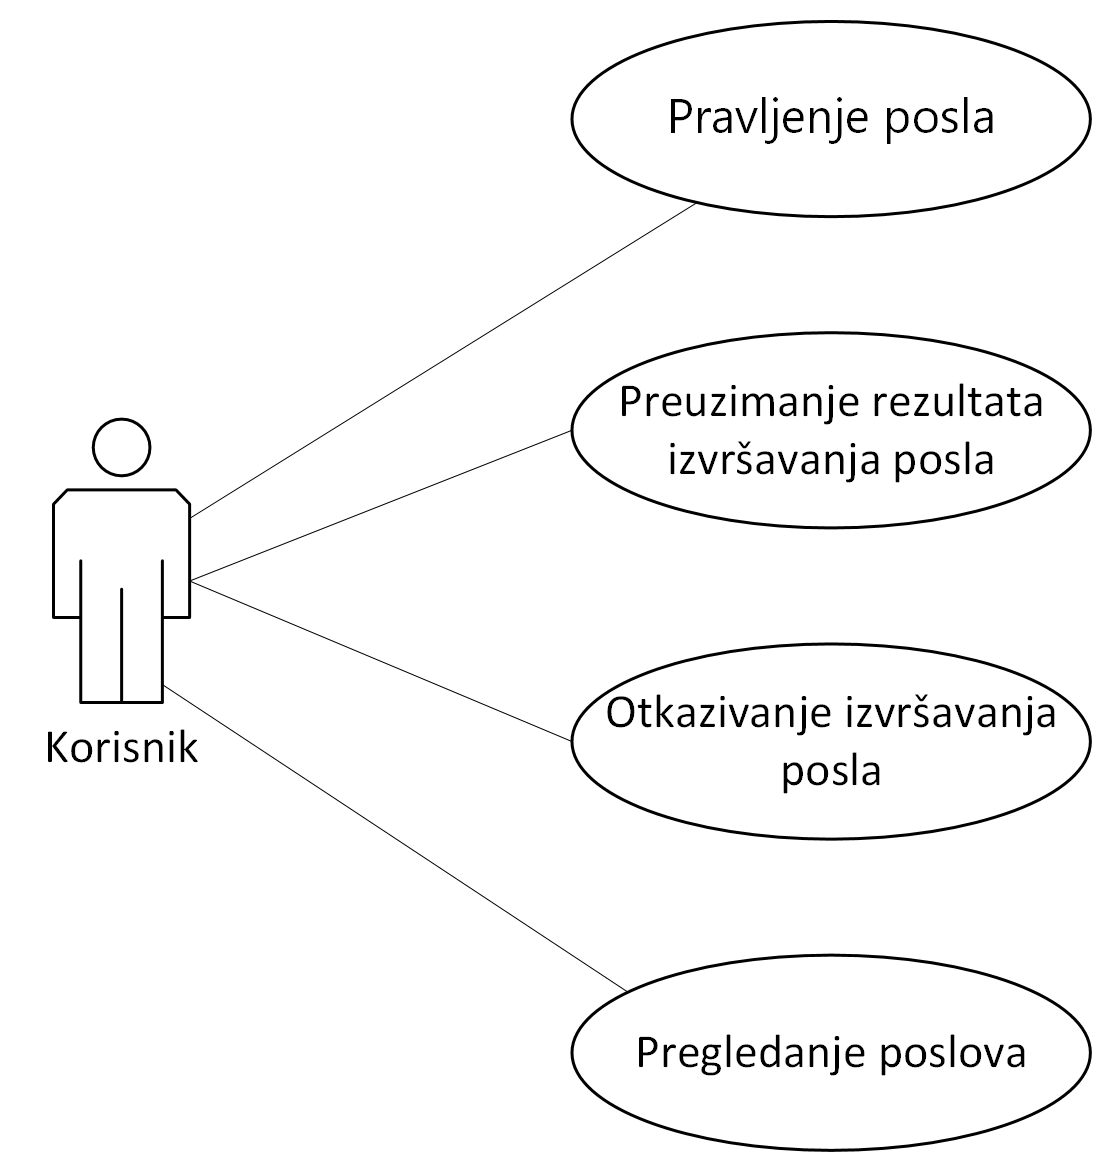
\includegraphics[width=0.6\textwidth]{./images/dijagram_slucajeva_upotrebe_korisnik.png}
  \caption{UML dijagram slučajeva upotrebe - Korisnik}
\end{figure}

% Zakazivanje
\subsection{Zakazivanje posla}
\begin{enumerate}
\item Naziv: Zakazivanje posla
\item Akter: Korisnik koji želi da izvrši posao nad ulaznim podacima
\item Kratak opis: Korisnik šalje zahtev za izvršavanje posla. Sistem validira zahtev i vraća potvrdu o uspešnosti zakazivanja.
\item Preduslovi: Korisnik ima neophodna prava da bi poslao zahtev sistemu. Sistem je u funkciji.
\item Postuslovi: Sistem je evidentirao novi zahtev za posao i prosledio ga na asinhrono izvršavanje.
\item Tok događaja:
	\begin{enumerate}
	\item \label{zak:konstruisezahtev}Korisnik konstruiše zahtev za izvršavanje posla. Zahtev se sastoji od:
		\begin{enumerate}
		\item Specifikacije željenog tipa posla,
		\item Niza ulaznih podataka
		\end{enumerate}
	\item \label{zak:saljezahtev} Korisnik šalje zahtev sistemu preko interneta koristeći predefinisani interfejs.
	\item \label{zak:proveraprava} Sistem proverava korisnikova prava.
	\item \label{zak:validacijazahteva} Sistem validira novopridošli zahtev za izvršavanje posla.
	\item Sistem evidentira novi zahtev za izvršavanje u bazi.
	\item \label{zak:asinhzakazivanje} Sistem stavlja zahtev u red za asinhrono izvršavanje.
	\item Korisnik dobija potvrdu da je posao zakazan i identifikator po kojem je posao zaveden u sistemu.
	\end{enumerate}
\item Alternativni tok događaja:
	\begin{enumerate}
	\item Korisnik nema prava da podnese zahtev. Ukoliko u koraku \ref{zak:proveraprava} korisnik nema neophodna prava, sistem odbija zahtev uz odgovarajuću grešku. Proces se nastavlja u koraku \ref{zak:saljezahtev} glavnog toka.
	\item Zahtev je nevalidan. Ukoliko u koraku \ref{zak:validacijazahteva} sistem prepozna nevalidan zahtev, odbija ga uz odgovarajuću grešku. Nevalidan zahtev može biti:
		\begin{enumerate}
		\item Nevalidna specifikacija tipa posla + tip posla mora biti podržan od strane sistema,
		\item Format ulaznih podataka nije odgovarajući.
		\end{enumerate}
Proces se nastavlja u koraku \ref{zak:konstruisezahtev} glavnog toka.
	\item Sistem je preopterećen i nema dovoljno resursa da zakaže novi posao. Ukoliko u koraku \ref{zak:asinhzakazivanje} sistem proceni da nema dovoljno resursa za izvršavanje posla, on odbija zahtev uz grešku da je sistem preopterećen i da korisnik pokuša kasnije. Proces se nastavlja u koraku \ref{zak:saljezahtev} glavnog toka.
	\end{enumerate}
\item Podtokovi: /
\item Specijalni zahtevi: Korisnik ima neophodno znanje za generisanje zahteva i korišćenje interfejsa sistema.
\item Dodatne informacije: /
\end{enumerate}

% Dohvatanje rezultata
\subsection{Preuzimanje rezultata posla}
\begin{enumerate}
\item Naziv: Preuzimanje rezultata posla
\item Akter: Korisnik koji želi da pruzme rezultate prethodno zakazanog posla
\item Kratak opis: Korisnik šalje zahtev za preuzimanje rezultata izvršavanja. Sistem validira zahtev i vraća tražene rezultate.
\item Preduslovi: Korisnik ima neophodna prava da bi poslao zahtev sistemu. Sistem je u funkciji. Posao je izvršen i rezultati su dostupni u bazi.
\item Postuslovi: Sistem je prosledio rezultate izvršavanja korisniku.
\item Tok događaja:
	\begin{enumerate}
	\item \label{rez:konstruisezahtev} Korisnik konstruiše zahtev za preuzimanje rezultata posla. Zahtev se sastoji od identifikatora posla za koji želi da preuzme rezultate.
	\item \label{rez:saljezahtev} Korisnik šalje zahtev sistemu preko interneta koristeći predefinisani interfejs.
	\item \label{rez:proveraprava} Sistem proverava korisnikova prava.
	\item \label{rez:validacijazahteva} Sistem validira novopridošli zahtev za preuzimanje rezultata posla.
	\item \label{rez:sinhslanjerez} Sistem šalje rezultate korisniku.
	\item Korisnik dobija rezultate.
	\end{enumerate}
\item Alternativni tok događaja:
	\begin{enumerate}
	\item Korisnik nema prava da podnese zahtev. Ukoliko u koraku \ref{rez:proveraprava} korisnik nema neophodna prava, sistem odbija zahtev uz odgovarajuću grešku. Proces se nastavlja u koraku \ref{rez:saljezahtev} glavnog toka.
	\item Zahtev je nevalidan. Ukoliko u koraku \ref{rez:validacijazahteva} sistem prepozna da posao sa datim identifikatorom ne postoji, odbija zahtev uz odgovarajuću grešku. Proces se nastavlja u koraku \ref{rez:konstruisezahtev} glavnog toka.
	\end{enumerate}
\item Podtokovi: /
\item Specijalni zahtevi: Korisnik ima neophodno znanje za generisanje zahteva i korišćenje interfejsa sistema.
\item Dodatne informacije: Ukoliko je posao uspešno izvršen, rezultat izvršavanja se sastoji od traženog rezultata izračunavanja. Ukoliko je posao neuspešno obrađen, rezultat se sastoji od informacije o grešci.
\end{enumerate}

% Otkazivanje
\subsection{Otkazivanje posla}
\begin{enumerate}
\item Naziv: Otkazivanje posla
\item Akter: Korisnik koji želi da otkaže prethodno zakazani posao
\item Kratak opis: Korisnik šalje zahtev za otkazivanje posla. Sistem validira zahtev i vraća potvrdu o uspešnosti otkazivanja.
\item Preduslovi: Korisnik ima neophodna prava da bi poslao zahtev sistemu. Sistem je u funkciji.
\item Postuslovi: Sistem je otkazao posao i obrisao evidenciju o poslu u bazi.
\item Tok događaja:
	\begin{enumerate}
	\item \label{otk:konstruisezahtev} Korisnik konstruiše zahtev za otkazivanje posla. Zahtev se sastoji od identifikatora posla koji želi da otkaže.
	\item \label{otk:saljezahtev} Korisnik šalje zahtev sistemu preko interneta koristeći predefinisani interfejs.
	\item \label{otk:proveraprava} Sistem proverava korisnikova prava.
	\item \label{otk:validacijazahteva} Sistem validira novopridošli zahtev za otkazivanje posla.
	\item \label{otk:sinhotkazivanje} Sistem sinhrono otkazuje sve operacije povezane sa poslom.
	\item Korisnik dobija potvrdu da je posao otkazan.
	\end{enumerate}
\item Alternativni tok događaja:
	\begin{enumerate}
	\item Korisnik nema prava da podnese zahtev. Ukoliko u koraku \ref{otk:proveraprava} korisnik nema neophodna prava, sistem odbija zahtev uz odgovarajuću grešku. Proces se nastavlja u koraku \ref{otk:saljezahtev} glavnog toka.
	\item Zahtev je nevalidan. Ukoliko u koraku \ref{otk:validacijazahteva} sistem prepozna da posao sa datim identifikatorom ne postoji ili nije aktivan, odbija zahtev uz odgovarajuću grešku. Proces se nastavlja u koraku \ref{otk:konstruisezahtev} glavnog toka.
	\end{enumerate}
\item Podtokovi: /
\item Specijalni zahtevi: Korisnik ima neophodno znanje za generisanje zahteva i korišćenje interfejsa sistema.
\item Dodatne informacije: /
\end{enumerate}

% Pregled poslova
\subsection{Pregled poslova}
\begin{enumerate}
\item Naziv: Pregled poslova
\item Akter: Korisnik koji želi da pruzme listu evidentiranih poslova u sistemu.
\item Kratak opis: Korisnik šalje zahtev za izlistavanje evidentiranih poslova. Sistem validira zahtev i vraća tražene informacije o evidentiranim poslovima.
\item Preduslovi: Korisnik ima neophodna prava da bi poslao zahtev sistemu. Sistem je u funkciji. Posao je izvršen i rezultati su dostupni u bazi.
\item Postuslovi: Sistem je prosledio rezultate izvršavanja korisniku.
\item Tok događaja:
	\begin{enumerate}
	\item \label{pregledp:konstruisezahtev} Korisnik konstruiše zahtev za izlistavanje poslova.
	\item \label{pregledp:saljezahtev} Korisnik šalje zahtev sistemu preko interneta koristeći predefinisani interfejs.
	\item \label{pregledp:proveraprava} Sistem proverava korisnikova prava.
	\item \label{pregledp:slanjeliste} Sistem šalje listu evidentiranih poslova dostupnih u bazi.
	\item Korisnik dobija listu evidentiranih poslova.
	\end{enumerate}
\item Alternativni tok događaja:
	\begin{enumerate}
	\item Korisnik nema prava da podnese zahtev. Ukoliko u koraku \ref{pregledp:proveraprava} korisnik nema neophodna prava, sistem odbija zahtev uz odgovarajuću grešku. Proces se nastavlja u koraku \ref{pregledp:saljezahtev} glavnog toka.
	\end{enumerate}
\item Podtokovi: /
\item Specijalni zahtevi: Korisnik ima neophodno znanje za generisanje zahteva i korišćenje interfejsa sistema.
\item Dodatne informacije: Rezultujuća lista poslova sadrži informacije o svakom evidentiranom poslu, i to:
	\begin{enumerate}
	\item Status posla
	\item Vreme početka zvršavanja posla
	\item Vreme završetka izvršavanja posla
	\end{enumerate}
\end{enumerate}

% Administratorovi slučajevi upotrebe
\section{Podešavanje sistema}
Dodatne funkcionalnosti sistema uključuju slučajeve upotrebe u kojima je učesnik administrator. Ovo uključuje podešavanje bezbednosti i prava pristupa sistemu, kao i prilagođavanje sistema da bude u u skladu sa korisnikovim korišćenjem, tj. opterećenosti sistema.

% Pristup podacima je ograničen i neophodno je da mogu da im pristupe samo autorizovane osobe.  -- prebaci negde

% AAD Admin
\subsection{Podešavanja prava pristupa}
Prava pristupa sistemu, tj. delovima sistema dodeljuje administrator bezbednosti. Prava pristupa pojedinačnim delovima sistema se kontrolišu kroz različta prava koja mogu biti dodeljena korisniku. Tipovi prava su:
	\begin{enumerate}
	\item Iskustvo krajnjeg korisnika - Mogućnost slanja zahteva sistemu kroz definisani javni interfejs,
	\item Pravo za praćenje rada sistema - Pristup telemetriji i logovima za praćenje rada sistema,
	\item Administrator klastera - Pristup klasteru za devops akcije,
	\item Administrator bezbednosti.
	\end{enumerate}
Slučajevi upotrebe iz ugla administratora za bezbednost su prikazani na slici \ref{fig:slucajupotrebe_aadadmin}. Detalji ovih slučajeva upotrebe su trivijana, te nisu opisani u nastavku.

\begin{figure}[!ht]
  \centering
  \label{fig:slucajupotrebe_aadadmin}
  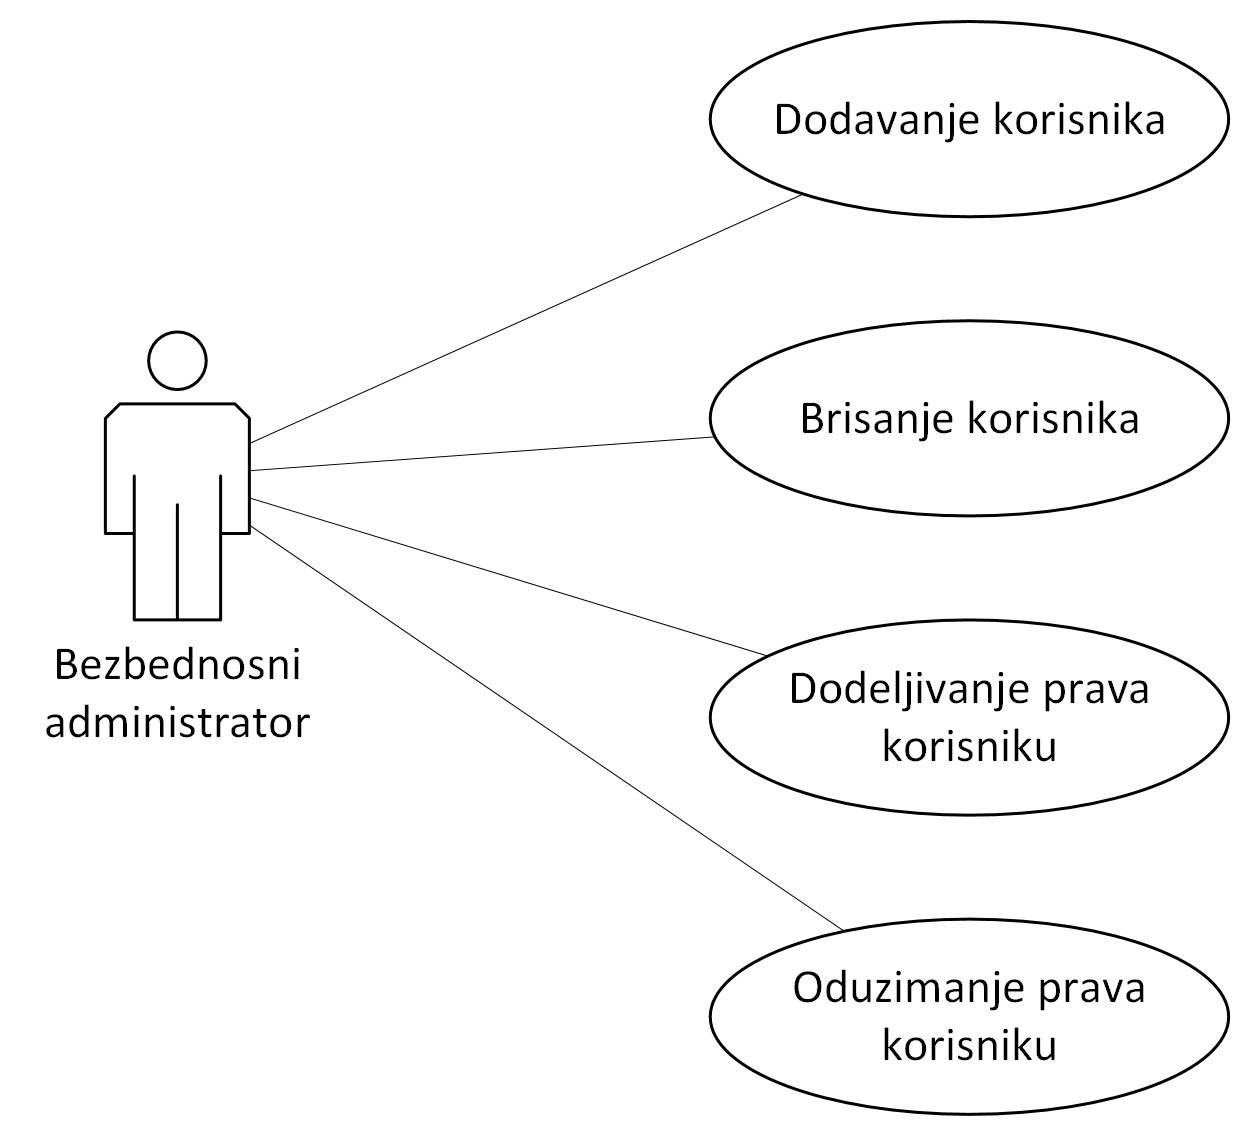
\includegraphics[width=0.6\textwidth]{./images/dijagram_slucajeva_upotrebe_administrator_sistema_aadadmin.png}
  \caption{UML dijagram slučajeva upotrebe - Administrator za bezbednost}
\end{figure}


% Podešavanje AKS klastera
\subsection{Podešavanje klastera}
Klaster administrator ima mogućnost da menja konfiguraciju sistema kako bi ga prilagodio korisnikovim zahtevima. To uključuje skaliranje sistema (menjanje broja jedinica za izvršavanje), kao i ažuriranje konfiguracije kojim se dodeljuju fizički resursi delovima sistema.
Slučajevi upotrebe iz ugla klaster administratora su prikazani na slici \ref{fig:slucajupotrebe_admin_klastera}. Detalji ovih slučajeva upotrebe su konceptualno jasni, a uključuju devops akcije, te nisu dalje razrađivani.

\begin{figure}[!ht]
  \centering
  \label{fig:slucajupotrebe_admin_klastera}
  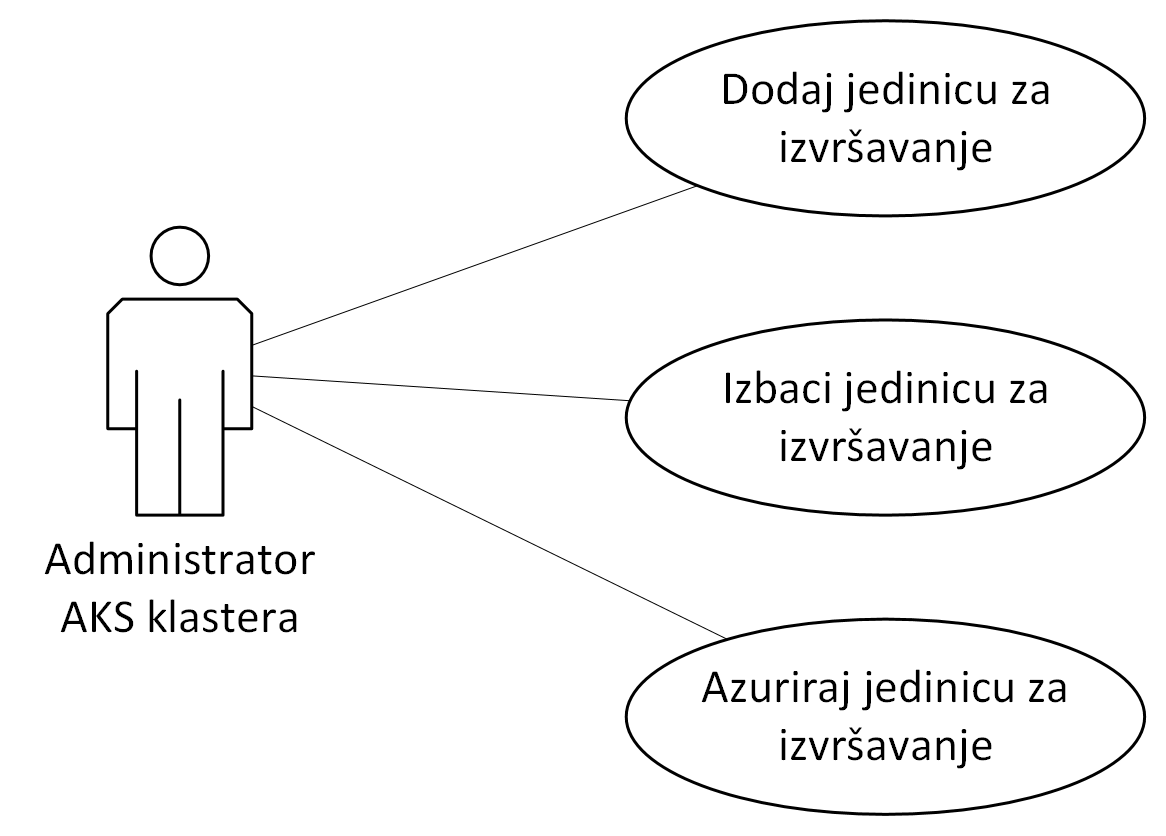
\includegraphics[width=0.6\textwidth]{./images/dijagram_slucajeva_upotrebe_administrator_klastera.png}
  \caption{UML dijagram slučajeva upotrebe - Klaster administrator}
\end{figure}

% ------------------------------------------------------------------------------
\chapter{Opis korišćenih tehnologija i alata}
\label{chp:opistehialata}
% ------------------------------------------------------------------------------

Za izradu programske realizacije sistema, korišćen je programski jezik C\#, i \emph{.NET Core 6.0} radni okvir. Korišćeno razvojno okruženje je eng. \emph{Microsoft Visual Studio 2022 - Community} i operativni sistem eng. \emph{Windows}.


\section{Doker kontejneri}
Izbor \emph{.NET Core} radnog okvira je omogućio pokretanje servisa u okviru Doker (eng. \emph{Docker}) kontejnera. 

TODO vise od docker kontejnerima

Postoji više prednosti ovog pristupa, a glavna je što čini servise lako prenosivim na različite platforme eng. \emph{Windows}, \emph{Mac} i \emph{Linux}. U realizaciji su koriškoristeći Linux kontejneri sa zapakovanim slikom (eng. \emph{image}) servisa.

Okruženje za lokalno pokretanje kontejnera eng \emph{Docker Desktop}



\section{Integracija sa Azure platformom}

\subsection{Azure Kubernetes Service}

\section{Kubernetes okrestrator}
TODO link ka zvaničnoj dokumentaciji i vise info o samom orkestratoru


% ------------------------------------------------------------------------------
\chapter{Implementacija}
\label{chp:impl}
% ------------------------------------------------------------------------------

U ovom poglavlju biće opisana implementacija sistema (eng. \emph{Distributed Computation System}).
Projekat je javno dostupan na servisu GitHub na adresi \href{https://github.com/milana-kovacevic/DistributedComputationSystem}{https://github.com/milana-kovacevic/DistributedComputationSystem}. Na adresi se takođe nalaze datoteke potrebne za kreiranje i konfiguraciju servisa pokrenutih u okviru Kubernetes klastera, kao i pomoćne skripte koje automatizuju proces postavljanja nove verzije aplikacija na klaster.


\section{Arhitektura sistema}

Arhitektura sistema je prikazana na slici \ref{fig:arhitektura}.

\begin{figure}[!ht]
  \centering
  \label{fig:arhitektura}
  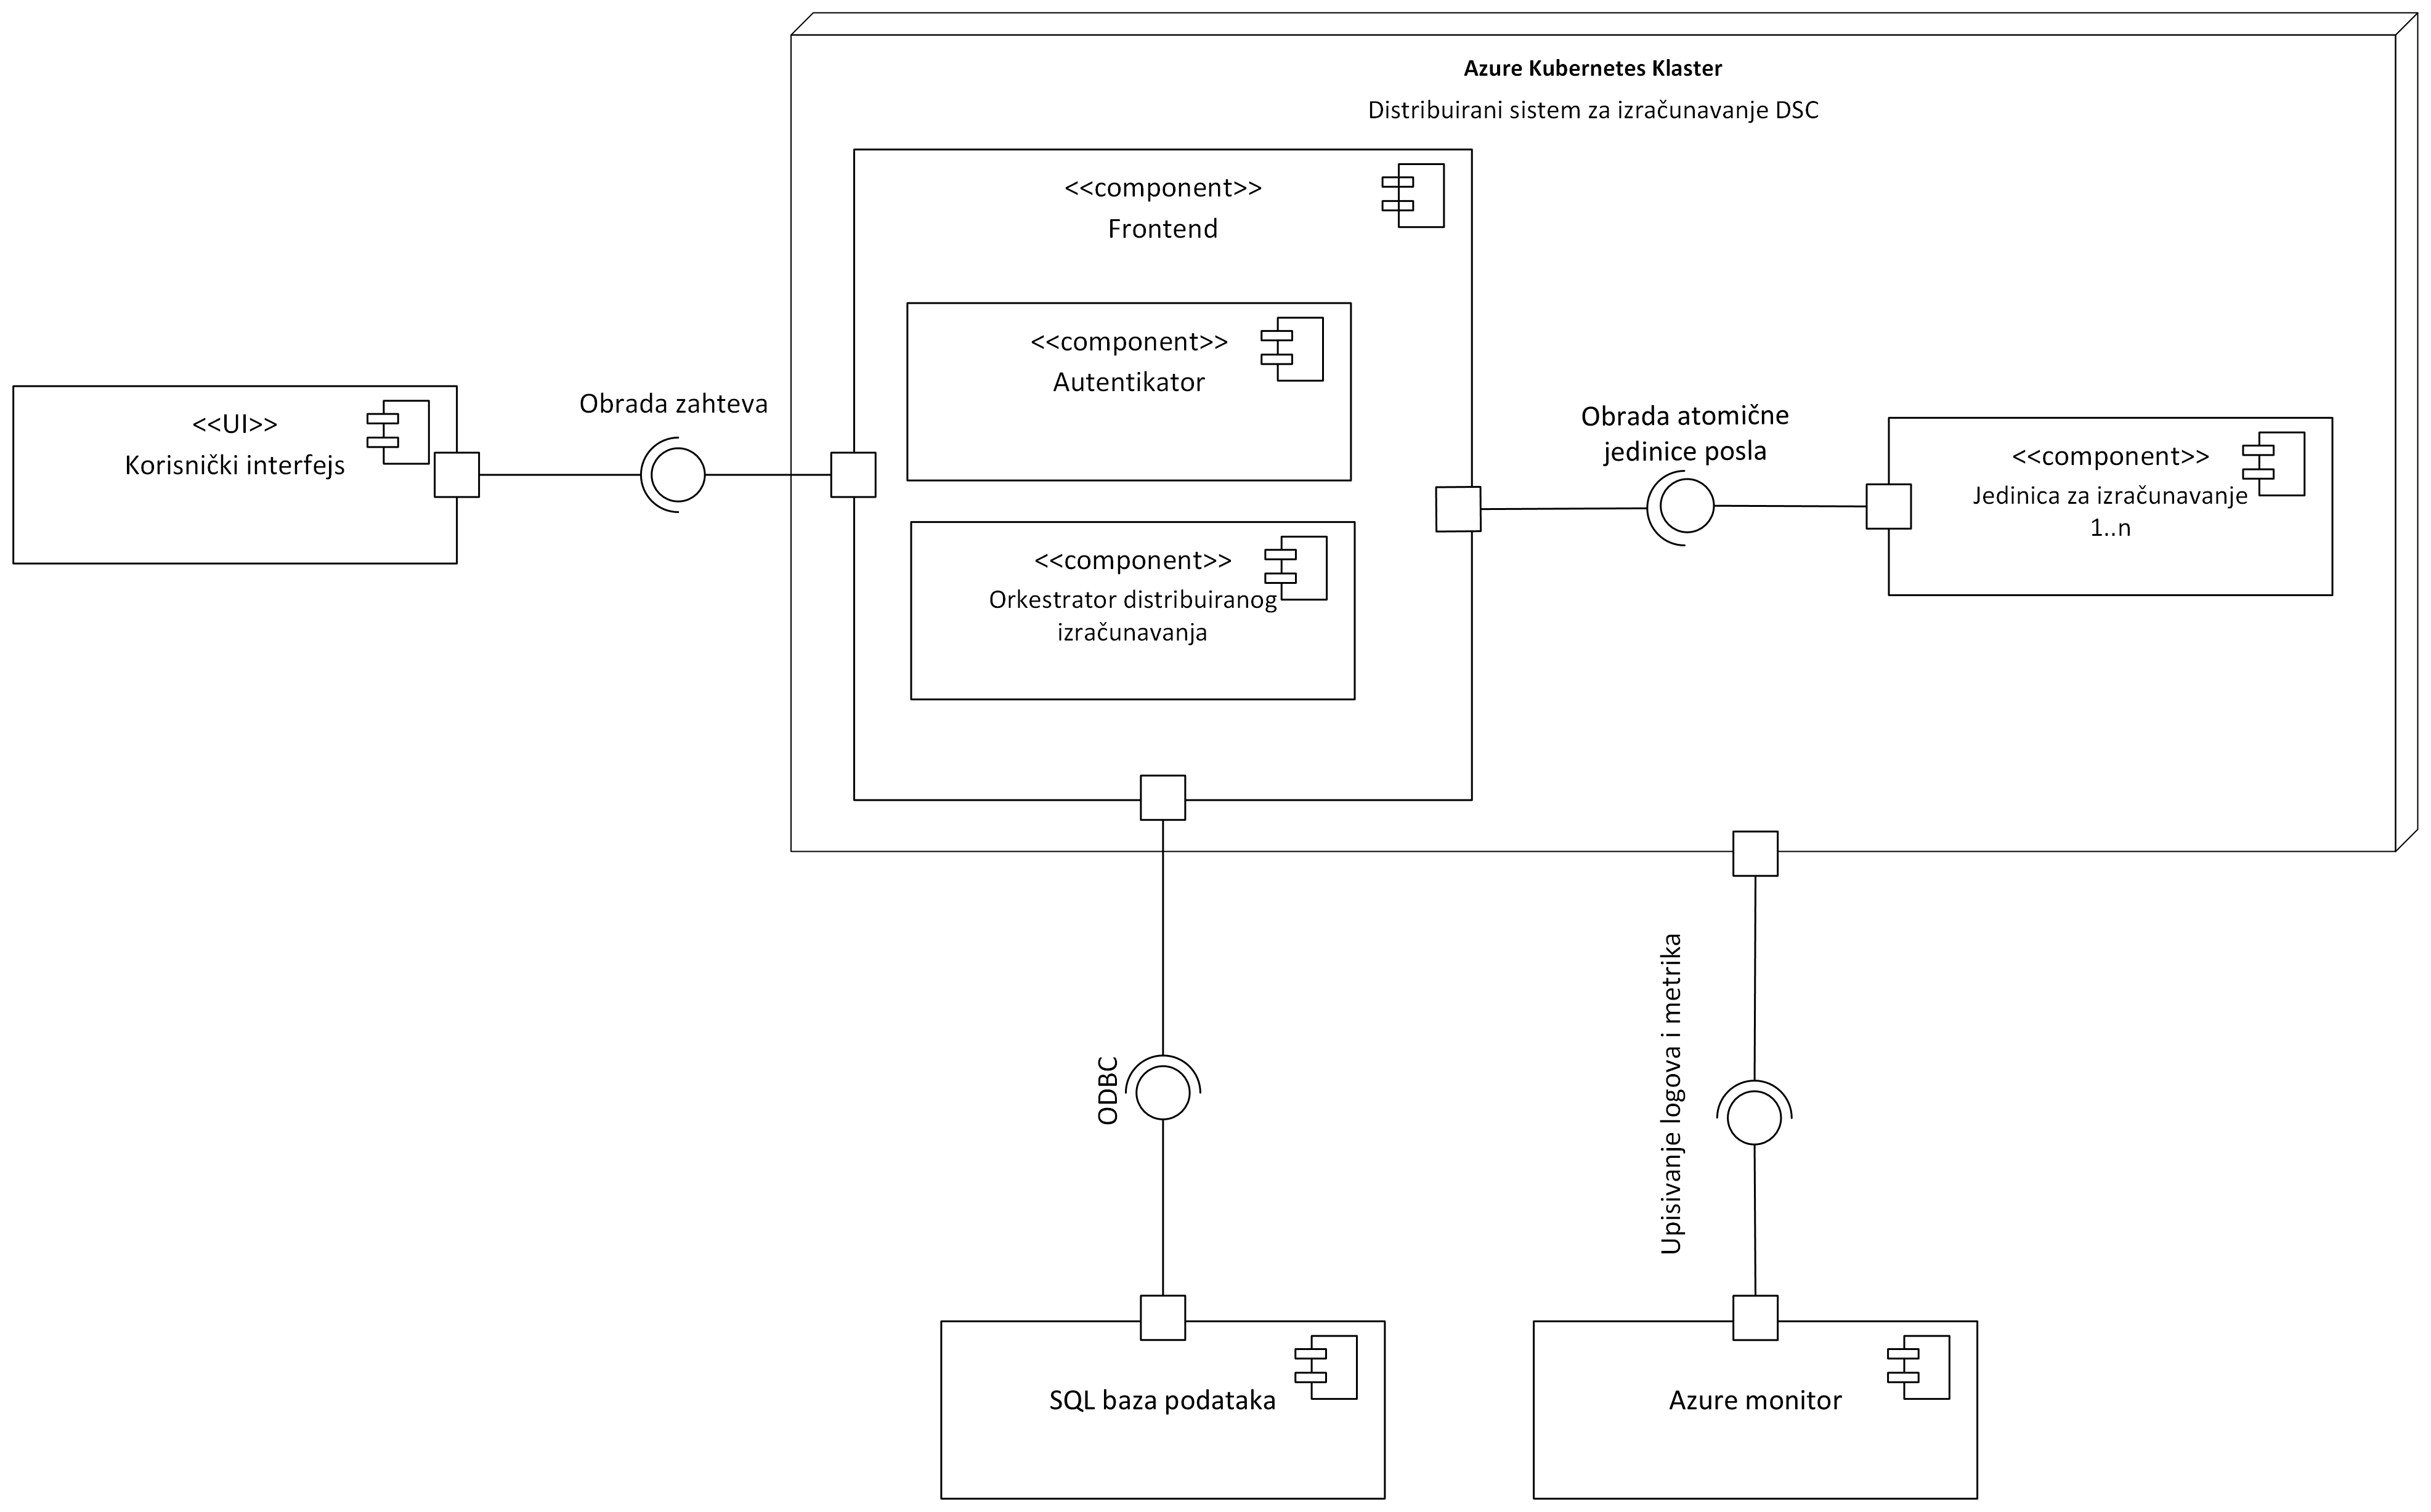
\includegraphics[width=1.0\textwidth]{./images/arhitektura_sistema_dijagram_komponenti.png}
  \caption{UML dijagram komponenti - Arhitektura sistema}
\end{figure}

Arhutekturalni obrazac korišćen prilikom razvoja pojedinačnih servisa sistema (Frontenda i Jedinice za izračunavanje) je Model-Pogled-Kontroler (eng. \emph{Model-View-Controller}), bez implementacije Pogled dela. Razlog za odabir ovog obrasca je što on uvodi podelu odgovornosti različitih delova servisa. Kontroler je okrenut ka spolja, i definiše interfejs za komunikaciju sa servisom. U slučaju Frontenda, on definiše API (eng. \emph{Application Programming Interface}) koji prima korisnikove zahteve za izvršavanje posla.

\section{Autentikacija}

Proces autentikacije je prikazan na slici \ref{fig:autentikacija}.

\begin{figure}[!ht]
  \centering
  \label{fig:autentikacija}
  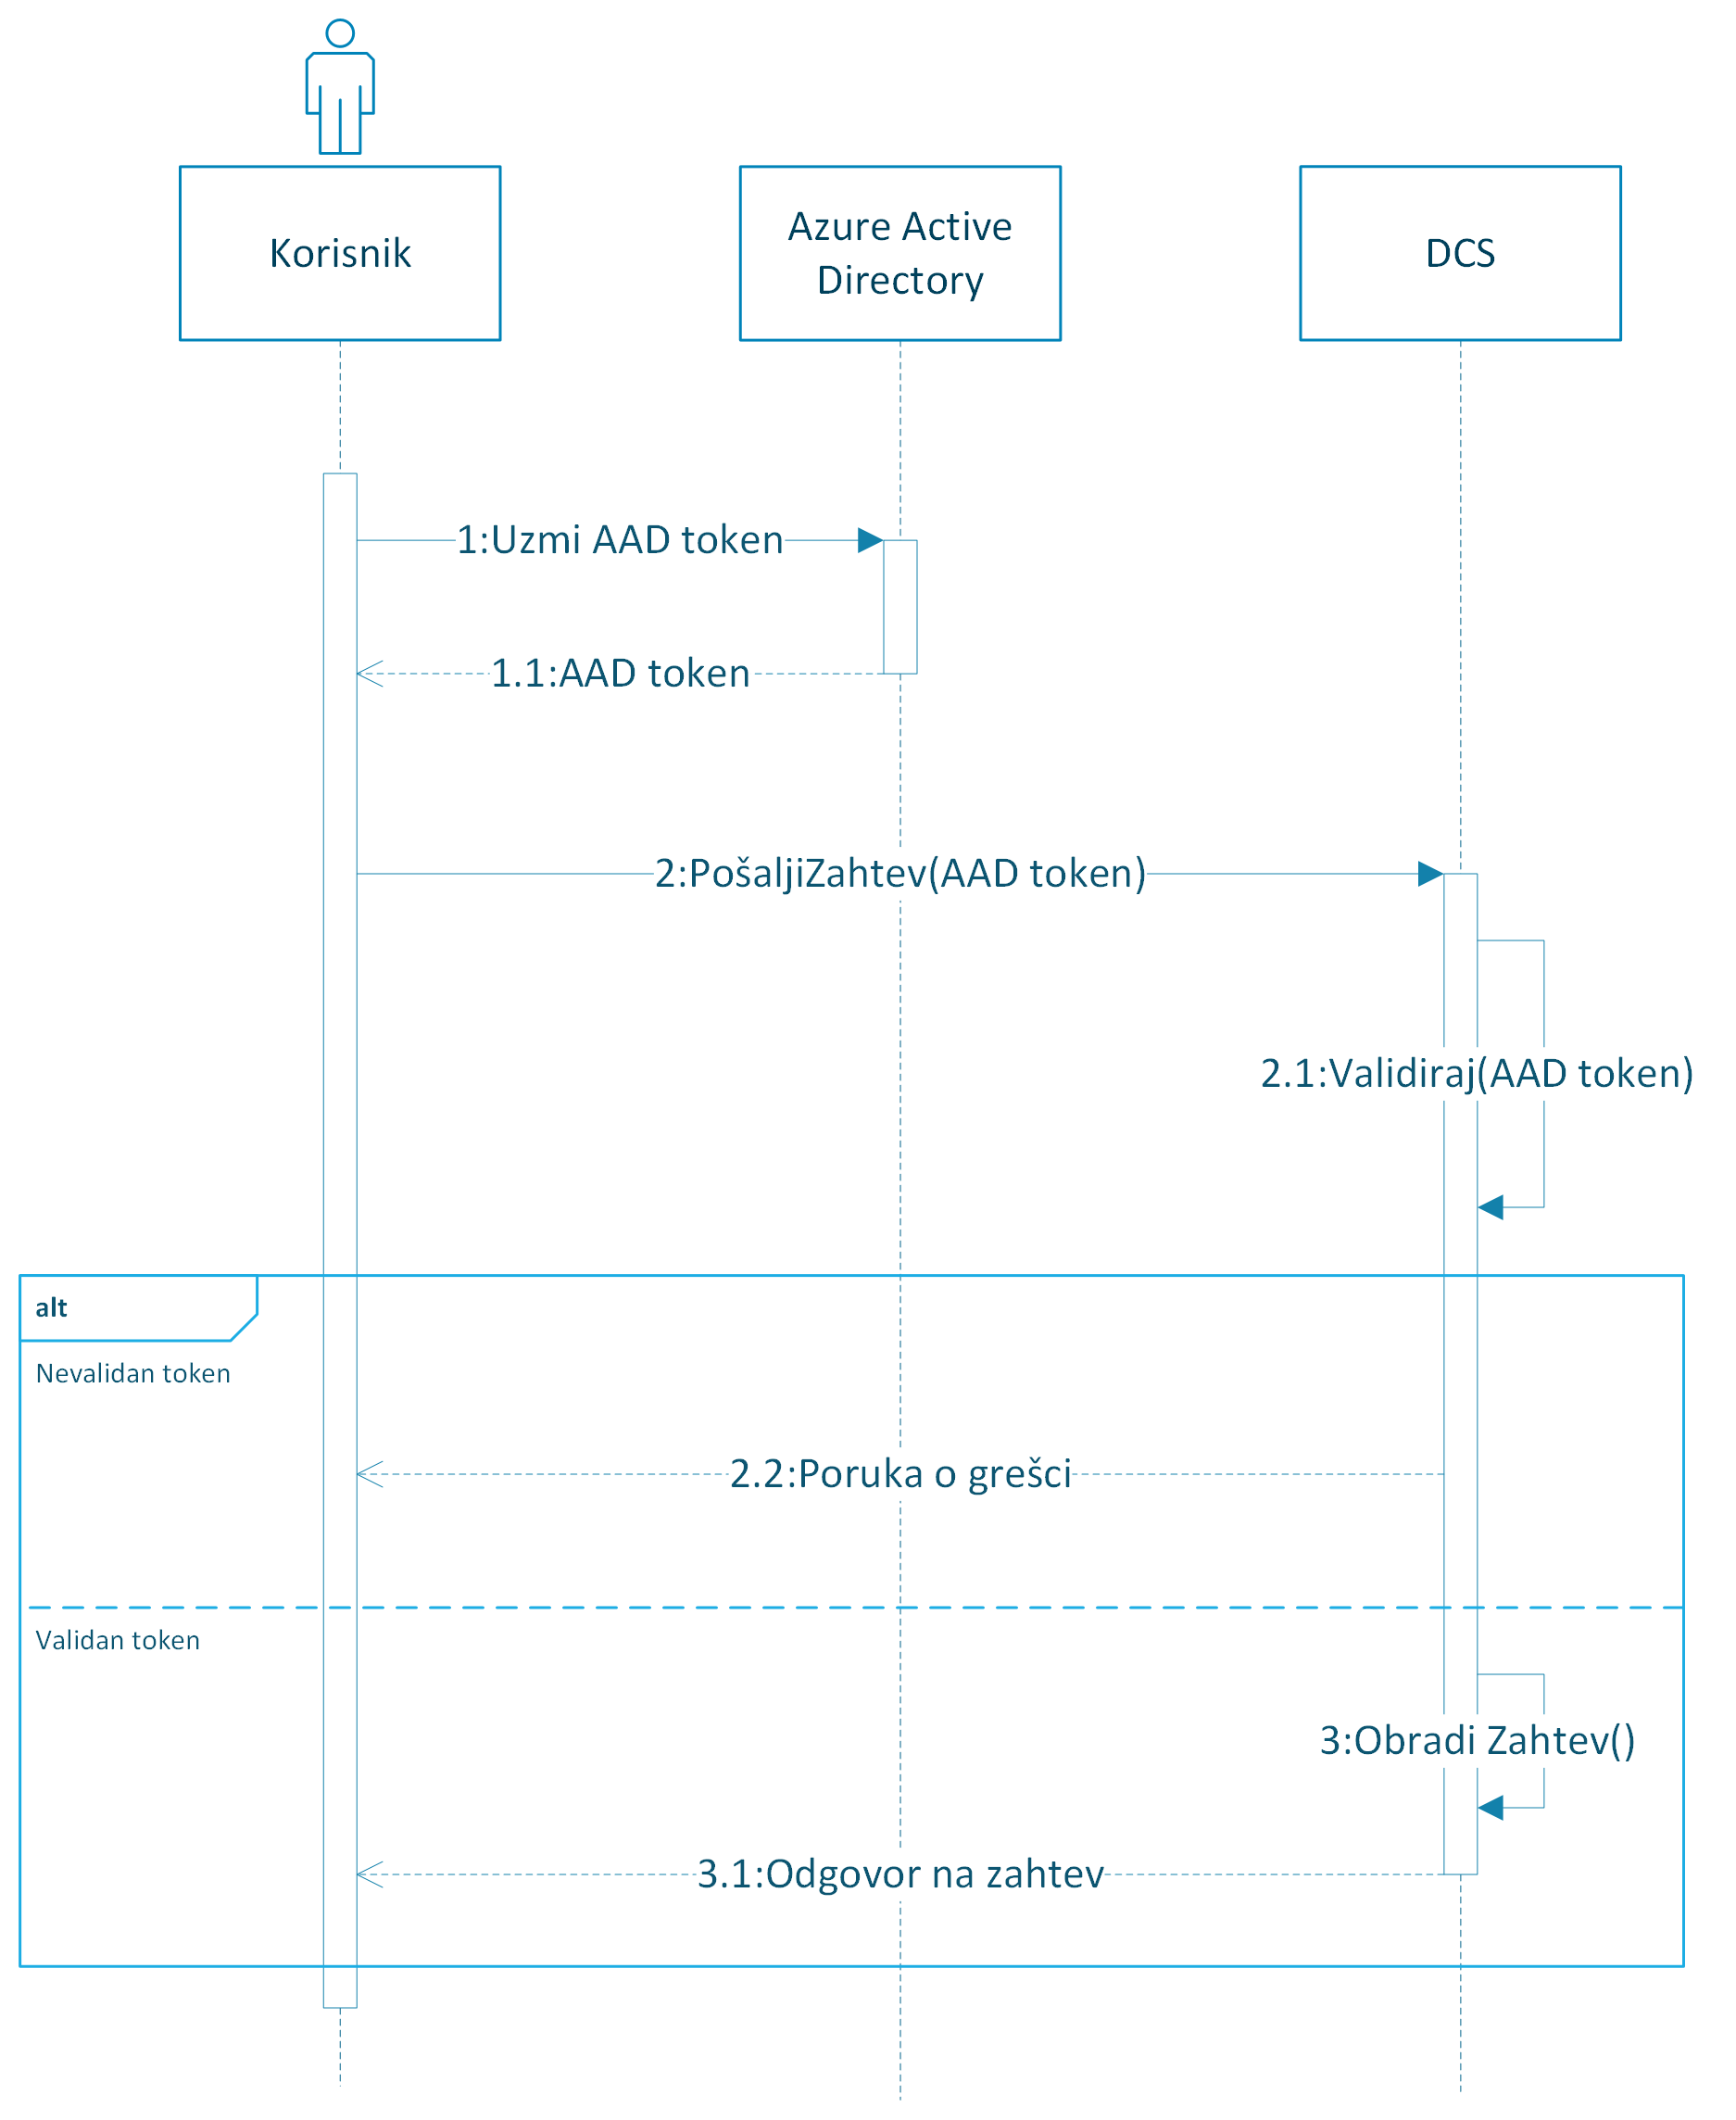
\includegraphics[width=1.0\textwidth]{./images/autentikacija_uml_dijagram_sekvence.png}
  \caption{UML dijagram sekvence - Autentikacija}
\end{figure}


\section{Baza}

ER (eng. \emph{Entity-Relation}) dijagram modela posla je prikazanan na slici \ref{fig:erposao}.

\begin{figure}[!ht]
  \centering
  \label{fig:erposao}
  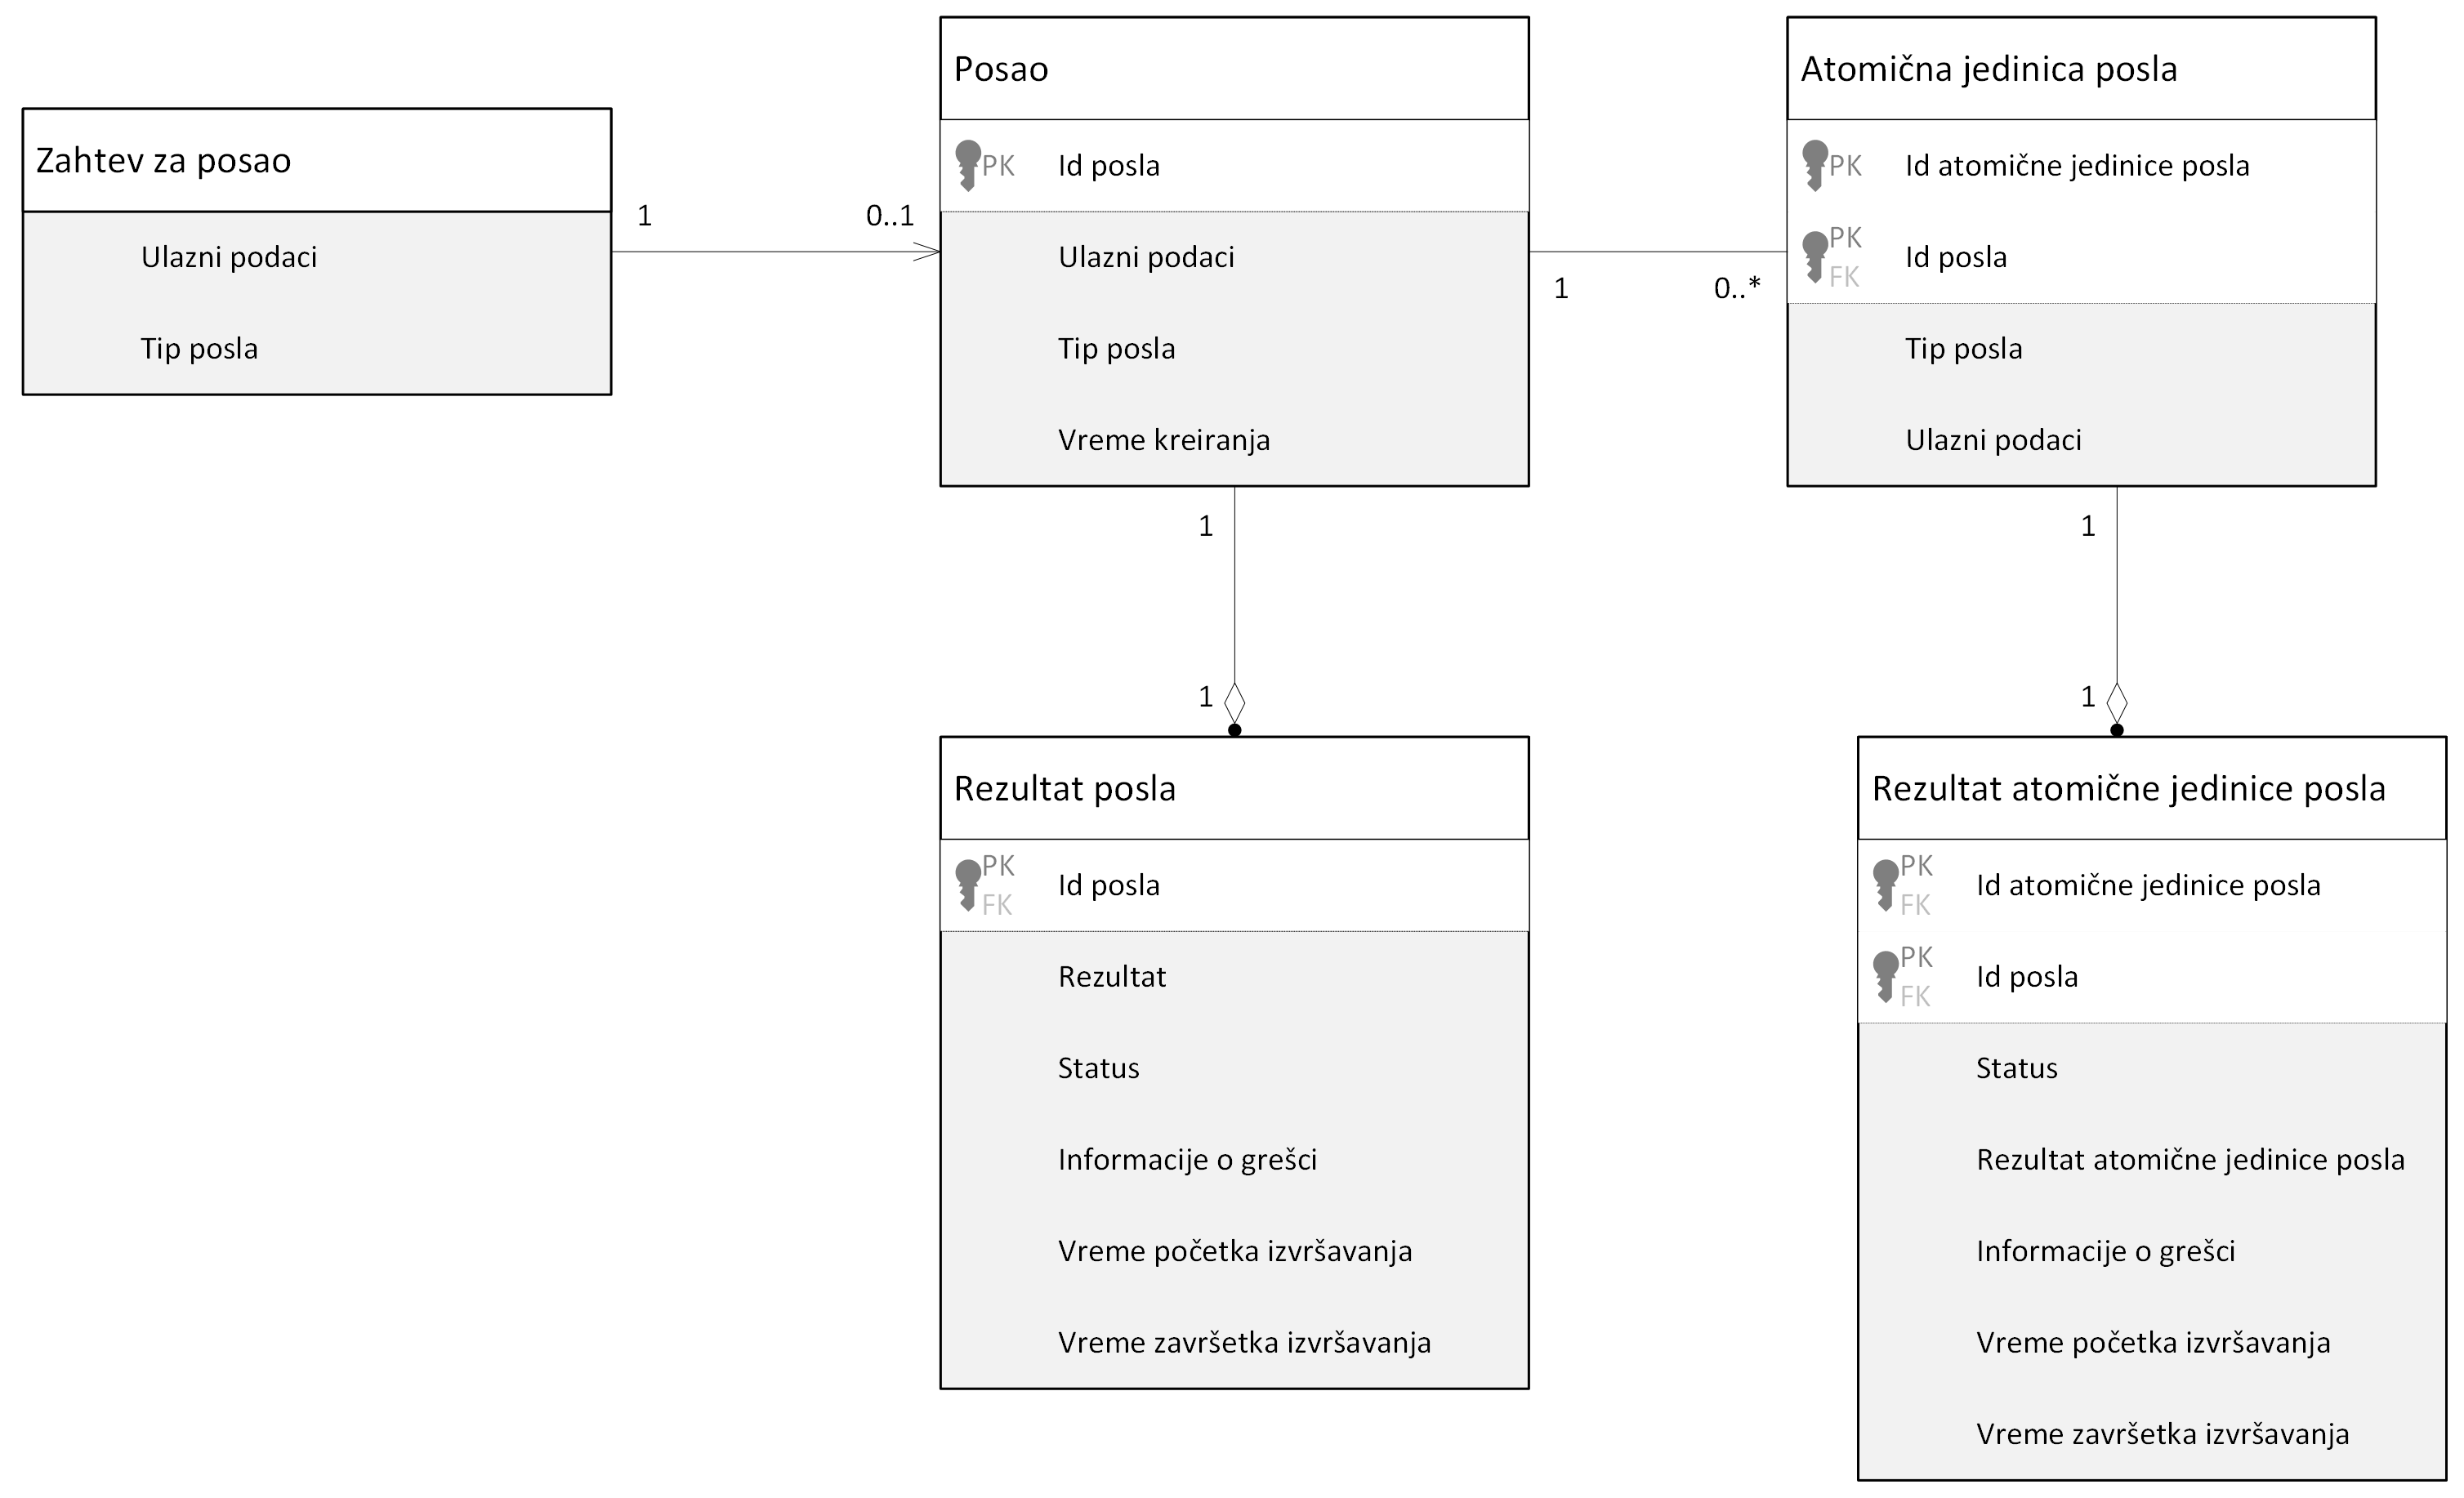
\includegraphics[width=1.0\textwidth]{./images/uml_er_dijagram_posao.png}
  \caption{ER dijagram entiteta - Posao}
\end{figure}



\section{Proces izvršavanja posla}
Stanja kroz koja prolazi posao su pikazana na slici \ref{fig:stanjaposla}.

\begin{figure}[!ht]
  \centering
  \label{fig:stanjaposla}
  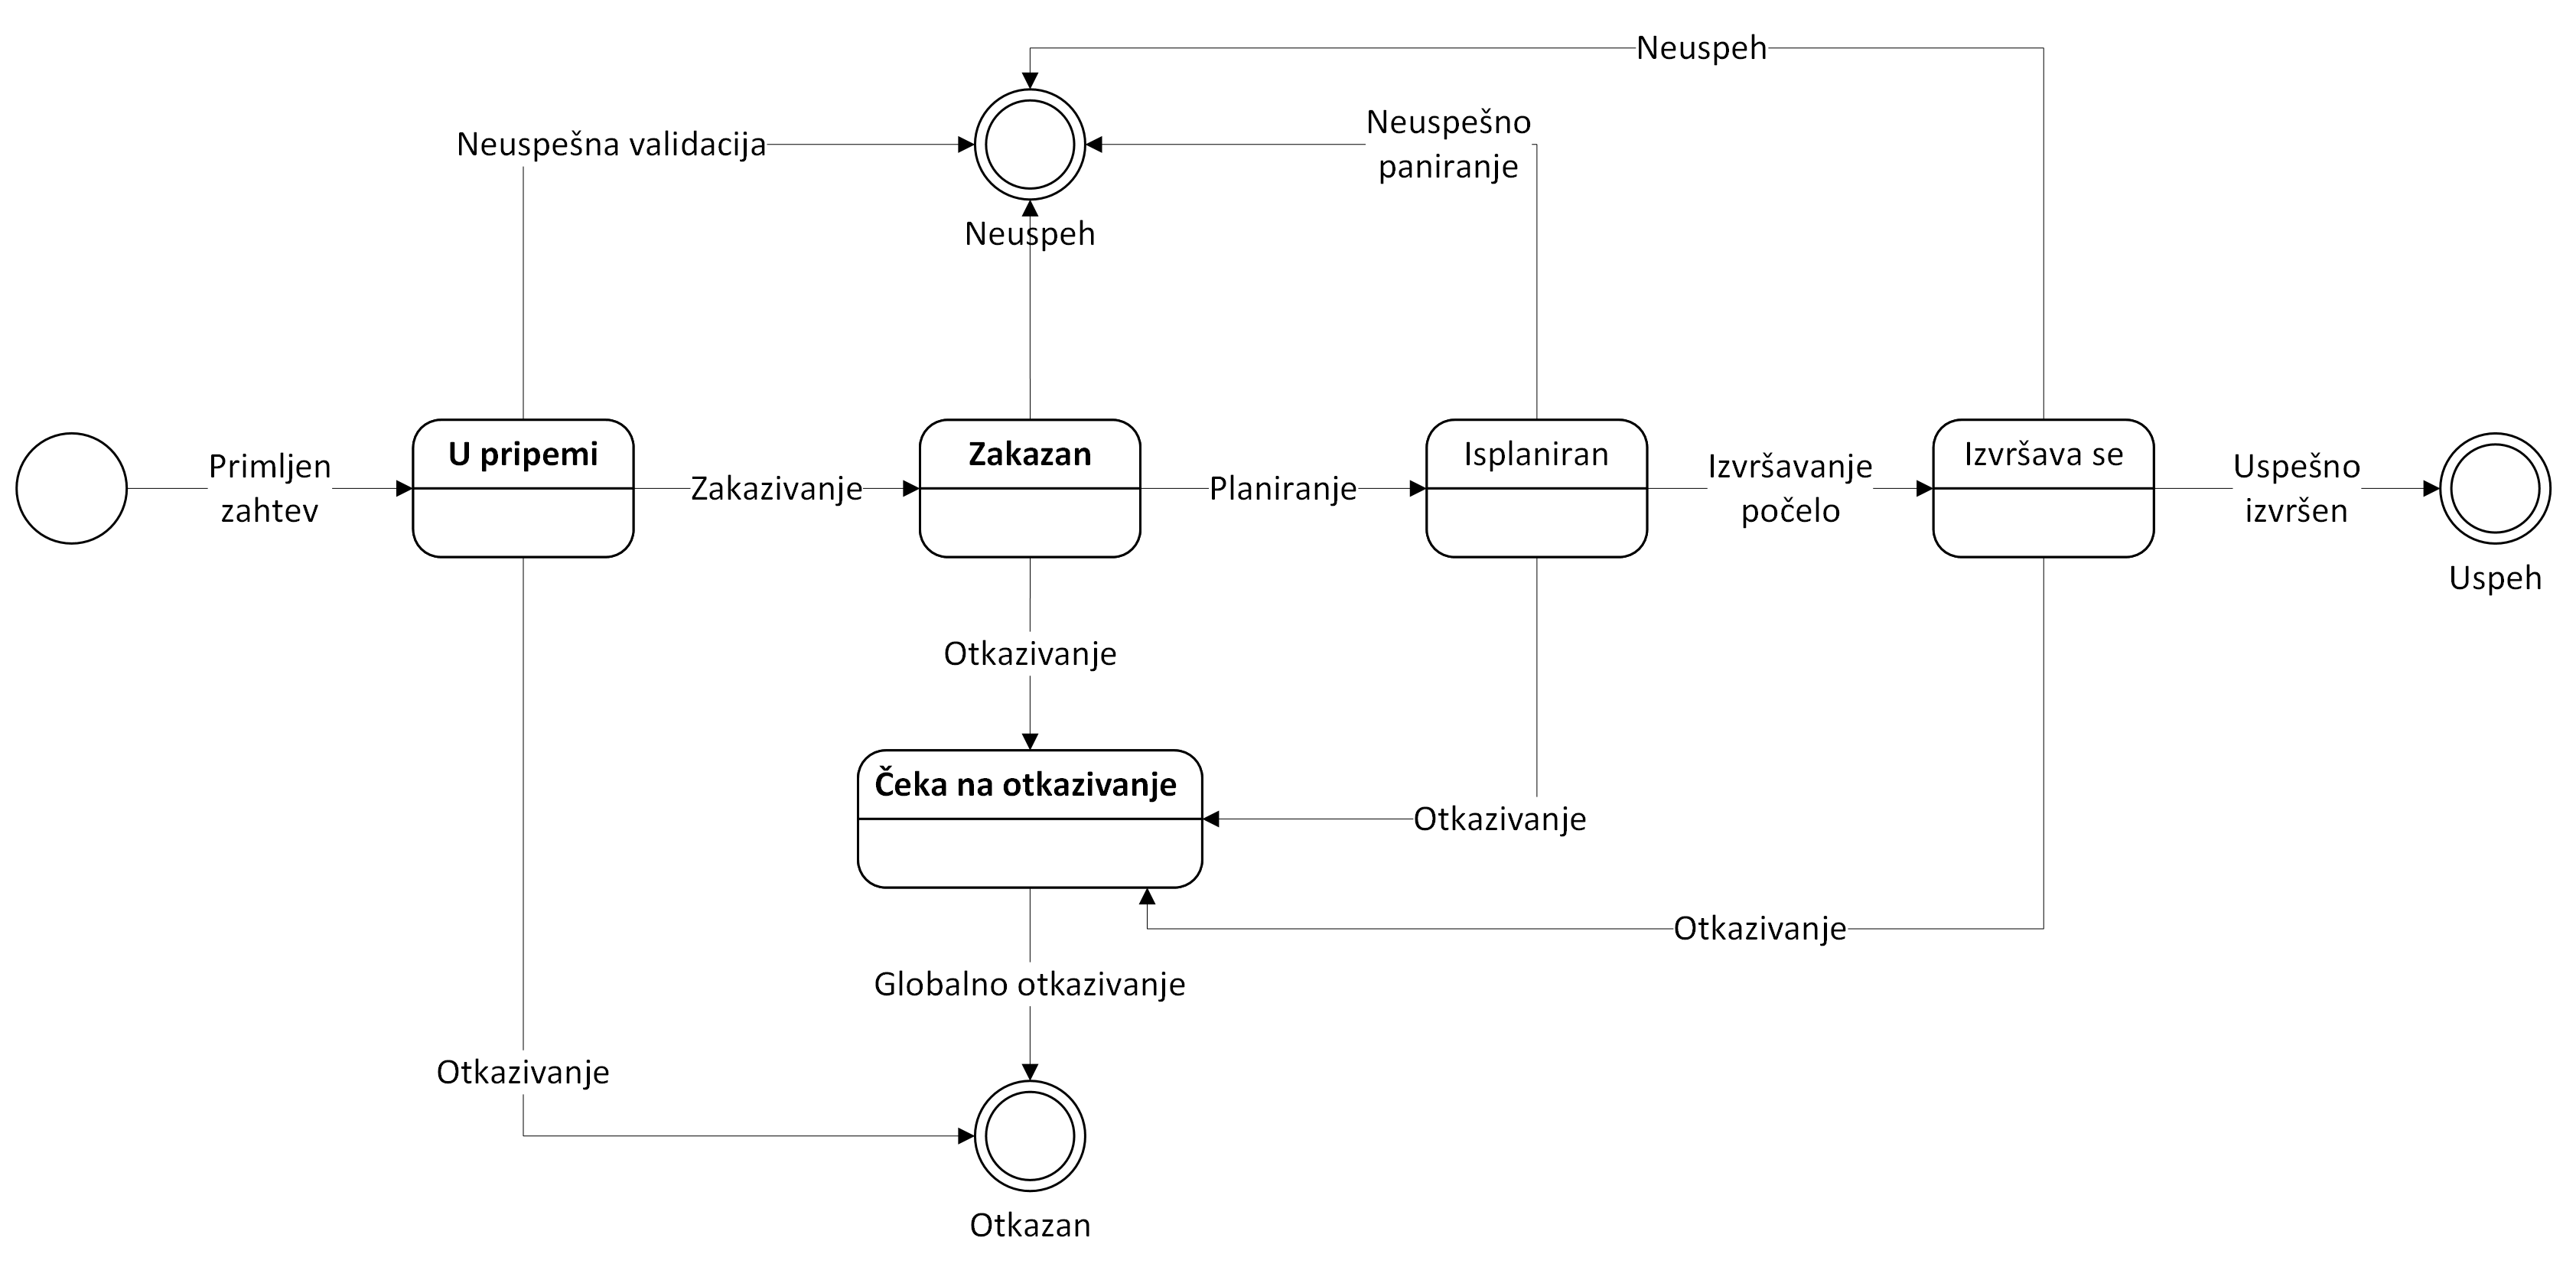
\includegraphics[width=1.0\textwidth]{./images/dijagram_stanja_posao.png}
  \caption{UML dijagram stanja - Posao}
\end{figure}


\section{Distribuiranje atomičnih jedinica posla}
TODO

\section{Pokretanje u oblaku}
TODO

% ------------------------------------------------------------------------------
\chapter{Testiranje sistema}
\label{chp:testiranjesistema}
% ------------------------------------------------------------------------------

Testiranje sistema TODO

\section{Unit testing}

\section{Functional testing}

% ------------------------------------------------------------------------------
\chapter{Praćenje metrika sistema}
\label{chp:pracenjemetrika}
% ------------------------------------------------------------------------------

Praćenje metrika sistema TODO

% ------------------------------------------------------------------------------
\chapter{Dalji razvoj sistema}
\label{chp:daljirazvoj}

% ------------------------------------------------------------------------------

Dalji razvoj sistema TODO


% ------------------------------------------------------------------------------
\chapter{Zaključak}
% ------------------------------------------------------------------------------
Zaključak, TODO

% ------------------------------------------------------------------------------
% Literatura
% ------------------------------------------------------------------------------
\literatura

% ==============================================================================
% Završni deo teze i prilozi
\backmatter
% ==============================================================================

% ------------------------------------------------------------------------------
% Biografija kandidata
\begin{biografija}
  \textbf{Milana Kovačević} je rođena u Zrenjaninu, 29. novembra 1995. godine. Osnovno i srednje obrazovanje (Zrenjaninska gimnazija, prirodno-matematički smer) završila je u rodnom gradu, uz sticanje diplome "Vuk Karadžić". Takođe je završila nižu muzičku školu, instrument klavir.
2014. godine je upisala osnovne studije na modulu Informatika na Matematičkom fakultetu Univerziteta u Beogradu. Osnovne studije je završila 2017. godine sa prosečnom ocenom 9.86, kao primalac stipendije Dositeja. Master akademske studije upisala je 2017. godine takođe na Matematičkom fakultetu na modulu Informatika. Položila je sve ispite predviđene planom i programom master akademskih studija sa prosečnom ocenom 9.15.

Nakon završetka osnovnih studija, nastavlja da se paralelno razvija i u industriji, radom u kompaniji Microsoft. Tokom rada se susreće sa sistemima za obradu i čuvanje podataka u okviru Azure plaforme, a radom na jednom od njih stiče i praktično znanje o distribuiranim sistemima i tehnologijama za rad u oblaku.

\end{biografija}
% ------------------------------------------------------------------------------

\end{document}
